\documentclass[a4paper,12pt]{article}

\usepackage{pdfpages}
\usepackage{parallel}
\usepackage[T2A]{fontenc}
\usepackage{ucs}
\usepackage[utf8x]{inputenc}
\usepackage[polish,english,russian]{babel}
\usepackage{hyperref}
\usepackage{rotating}
\usepackage[inner=2cm,top=1.8cm,outer=2cm,bottom=2.3cm,nohead]{geometry}
\usepackage{listings}
\usepackage{graphicx}
\usepackage{wrapfig}
\usepackage{longtable}
\usepackage{indentfirst}
\usepackage{array}
\newcolumntype{P}[1]{>{\raggedright\arraybackslash}p{#1}}
\frenchspacing
\usepackage{fixltx2e} %text sub- and superscripts
\usepackage{icomma} % коскі ў матэматычным рэжыме
\PreloadUnicodePage{4}

\newcommand{\longpage}{\enlargethispage{\baselineskip}}
\newcommand{\shortpage}{\enlargethispage{-\baselineskip}}

\def\switchlang#1{\expandafter\csname switchlang#1\endcsname}
\def\switchlangbe{
\let\saverefname=\refname%
\def\refname{Літаратура}%
\def\figurename{Іл.}%
}
\def\switchlangen{
\let\saverefname=\refname%
\def\refname{References}%
\def\figurename{Fig.}%
}
\def\switchlangru{
\let\saverefname=\refname%
\let\savefigurename=\figurename%
\def\refname{Литература}%
\def\figurename{Рис.}%
}

\hyphenation{admi-ni-stra-tive}
\hyphenation{ex-pe-ri-ence}
\hyphenation{fle-xi-bi-li-ty}
\hyphenation{Py-thon}
\hyphenation{ma-the-ma-ti-cal}
\hyphenation{re-ported}
\hyphenation{imp-le-menta-tions}
\hyphenation{pro-vides}
\hyphenation{en-gi-neering}
\hyphenation{com-pa-ti-bi-li-ty}
\hyphenation{im-pos-sible}
\hyphenation{desk-top}
\hyphenation{elec-tro-nic}
\hyphenation{com-pa-ny}
\hyphenation{de-ve-lop-ment}
\hyphenation{de-ve-loping}
\hyphenation{de-ve-lop}
\hyphenation{da-ta-ba-se}
\hyphenation{plat-forms}
\hyphenation{or-ga-ni-za-tion}
\hyphenation{pro-gramming}
\hyphenation{in-stru-ments}
\hyphenation{Li-nux}
\hyphenation{sour-ce}
\hyphenation{en-vi-ron-ment}
\hyphenation{Te-le-pathy}
\hyphenation{Li-nux-ov-ka}
\hyphenation{Open-BSD}
\hyphenation{Free-BSD}
\hyphenation{men-ti-on-ed}
\hyphenation{app-li-ca-tion}

\def\progref!#1!{\texttt{#1}}
\renewcommand{\arraystretch}{2} %Іначай формулы ў матрыцы зліпаюцца з лініямі
\usepackage{array}

\def\interview #1 (#2), #3, #4, #5\par{

\section[#1, #3, #4]{#1 -- #3, #4}
\def\qname{LVEE}
\def\aname{#1}
\def\q ##1\par{{\noindent \bf \qname: ##1 }\par}
\def\a{{\noindent \bf \aname: } \def\qname{L}\def\aname{#2}}
}

\def\interview* #1 (#2), #3, #4, #5\par{

\section*{#1\\{\small\rm #3, #4. #5}}

\def\qname{LVEE}
\def\aname{#1}
\def\q ##1\par{{\noindent \bf \qname: ##1 }\par}
\def\a{{\noindent \bf \aname: } \def\qname{L}\def\aname{#2}}
}

\lstset{language=Python}

\renewcommand{\arraystretch}{2} %Іначай формулы ў матрыцы зліпаюцца з лініямі

% To be edited when needed %%%%%%%%%%
\newcommand{\progname}{\textit} % Стыль адлюстравання імёнаў праграм
\newcommand{\aknowl}{\textit} % Стыль для падзяк
%%%%%%%%%%%%%%%%%%%%%%%%%%%%%%%%%%%%%

\begin{document}

\renewcommand{\figurename}{Рыс.} % Не перакідаць у прэамбулу --- не працуе, чаму -- халера ведае.
\renewcommand{\abstractname}{Анатацыя}
\renewcommand{\refname}{Літаратура}

\title{Шляхі акселерацыі выканання вылічальнай нагрузкі на Python}
\author{Антон Літвіненка\\ \small Кіеўскі нацыянальны ўніверсітэт імя Тараса Шаўчэнкі\\ \small \texttt{tenebrosus.scriptor@gmail.com}}
\date{}
\maketitle

\begin{abstract}
Interpreted programming languages are known for their fle\-xibility and convenience, but suffer from low execution speed comparing to compiled ones. However, they find a use for time-consuming applications. The enhanced methods of acceleration for interpreted languages are available, first of all just-in-time (JIT) compilation. The effect of the JIT compilation on the execution speed of a time-consuming scientific program is re\-ported, and a few imp\-le\-mentations of JIT compilers for Python are compared. \progname{PyPy} was found to be the fastest one, \progname{Psyco} --- slightly slower, \progname{Unladen Swallow} --- nearly useless.
\end{abstract}

Інтэрпрэтаваныя мовы праграмавання ўсё часцей ужываюцца пры напісанні праграм для разнастайных сфераў дастасавання, у тым ліку такіх, што традыцыйна не асацыююцца з інтэрпрэтаванымі мовамі, а менавіта "--- напісанне праграм, якія патрабуюць вялікіх вылічальных рэсурсаў.

Так, напрыклад, існуе часткова напісаная на Python бібліятэка для квантавахімічнага мадэлявання \progname{pDynamo} \cite{pDynamo}, аўтары якой адмовіліся ад традыцыйнага ў гэтай галіне выбару між Fortran, C або C++ і сваіх ранейшых напрацовак на Fortran, і аддалі перавагу інтэрфейсу на Python (з рэалізацыяй найбольш крытычнай да хуткасці часткі коду на C). Прычыны поспехаў інтэрпрэтаваных моў у гэтай галіне ў выпадку навуковых праграм, верагодна, абумоўленыя лёгкасцю распрацоўкі для неадмыслоўцаў.

Таксама гэтыя мовы зручнейшыя для распрацоўкі з элементамі рэфлектыўнага праграмавання (калі праграме неабходна генераваць частку ўласнага коду).

Аўтарам дакладу была распрацаваная праграма \progname{Mj{\"o}llnir}, якая выконвае інтэрпрэтацыю вынікаў магнетахімічнага эксперыменту з выкарыстаннем паўнаматрычнага метаду рашэння аператарных ураўненняў для спін"=гамільтаніяна магнітных узаемадзеянняў, зыходзячы з мадэлі, якая задаецца карыстальнікам \cite{Mjollnir}. Для рашэння гэтае задачы неабходна на падставе мадэлі пабудаваць матрыцы спін"=гамільтаніяна (прыклад на рыс.~\ref{fig:spin_ham}), прычым у алгебраічным (сімвальным) выглядзе. Алгарытм пабудовы быў рэалізаваны на Python. Праграму можна атрымаць ад аўтара пад умовамі ліцэнзіі GNU GPL v3.

Безумоўна, праблема хуткасці выканання ў такім выпадку становіцца актуальнай.

\begin{figure}[ht]
$$
\left(
\begin{array}{c|cccc}
z &|+\frac{1}{2};+\frac{1}{2}\rangle&|+\frac{1}{2};-\frac{1}{2}\rangle&|-\frac{1}{2};+\frac{1}{2}\rangle&|-\frac{1}{2};-\frac{1}{2}\rangle\\
\hline
\langle+\frac{1}{2};+\frac{1}{2}|& \mu H_z g_z-\frac{1}{2}J_z & 0 & 0 & 0\\
\langle+\frac{1}{2};-\frac{1}{2}|& 0 & \frac{1}{2}J_z  & -J_z & 0\\
\langle-\frac{1}{2};+\frac{1}{2}|& 0 & -J_z & \frac{1}{2}J_z & 0\\
\langle-\frac{1}{2};-\frac{1}{2}|& 0 & 0 & 0 & -\mu H_zg_z-\frac{1}{2}J_z\\
\end{array}
\right)
$$
\caption{Матрыца спін-гамільтаніяна для асі $z$ для комплексу Cu\textsubscript{2}.}
\label{fig:spin_ham}
\end{figure}

Метады акселерацыі выканання прадугледжваюць адыход ад чыстай інтэрпрэтацыі зыходнага коду ў момант выканання і пераход да разнастайных гібрыдных схемаў трансляцыі.

Па-першае, самая крытычная да рэсурсаў частка функцыянальнасці можа быць напісаная на кампіляванай мове праграмавання. Але такі падыход патрабуе перапісвання коду і можа ўскладняць рэалізацыю.

Ускосным дастасаваннем такога падыходу з'яўляецца выкарыстанне адных канструкцый мовы замест іншых, аналагічных, але хутчэйшых\cite{Optimize}.  Так, сапраўды, інструкцыя:
\begin{verbatim}
    map(operator.add, l1, l2) 
\end{verbatim}
хутчэй, чым:
\begin{verbatim}
    map(lambda x,y: x+y, l1, l2)
\end{verbatim}
 А спроба сабраць матрыцу ў адзін радок інструкцыяй:
\begin{verbatim}
    collect_str+=a[i][j]  
\end{verbatim}
 у цыкле істотна прайграе інструкцыі:
\begin{verbatim} 
    "".join(map(lambda x:"".join(x),a)).
\end{verbatim}
У той жа час, неабходна дакладна ведаць спосабы рэалізацыі тых ці іншых інструкцый (якія могуць змяняцца з часам і залежаць ад рэалізацыі).

Прэкампіляцыя ў байт"=код з'яўляецца традыцыйнай і выкарыстоўваецца заўсёды, калі ёсць такая мажлівасць.

Існуюць праекты статычных кампілятараў падмноства мовы Python у машынны код, напрыклад, \progname{Shedskin}. Праект \progname{PyPy}, акрамя іншых дастасаванняў, здольны статычна кампіляваць г.зв. падмноства RPython. На жаль, гэты падыход абмяжоўвае мажлівасці мовы (у прыватнасці, яго складана ўжыць для ўжо гатовага коду).

Найбольш цікавымі з'яўляюцца праекты JIT-кампілятараў:
\begin{itemize}
\item Модуль \progname{Psyco}. Рэалізаваны як модуль \progname{CPython} (стандартнае рэалізацыі мовы). З'яўляецца найбольш старым, вядомым, \linebreak зручным, а да апошняга часу "--- і самым хуткім. Недахопы: прывязаны да версіі інтэрпрэтатара і платформы (толькі x86), прычым распрацоўка новых версій ускладненая (напрыклад, версіі пад Python 2.7 няма дагэтуль).

\item Праект \progname{PyPy}. З'яўляецца інтэпрэтатарам і JIT"=кампілятарам. Хуткасць выканання расце ад версіі да версіі і ўжо перавышае хуткасць Psyco \cite{speed}. Ускладненая праца з вонкавымі бібліятэкамі на C.

\item Праект \progname{Unladen Swallow}. Пазіцыянуецца як аптымізаваны \linebreak \progname{CPython} з JIT-кампіляцыяй. Пакуль што працуе нашмат павольней за папярэднія два.
\end{itemize}

Агульная праблема ўсіх JIT"=рэалізацый "--- патрабаванне большага аб'ёму памяці, чым \progname{CPython}.
Вынікі сінтэтычных тэстаў хуткасці наяўныя ў Сеціве \cite{speed}. Для праверкі эфекту акселерацыі ў выпадку праграмы \progname{Mj{\"o}llnir} былі выкананыя тэсты для біядзернага комплексу медзі (Cu\textsubscript{2}, 4 базісныя функцыі), трыядзернага Fe\textsubscript{2}Co (432) і 4-ядзернага Mn\textsubscript{4} (625). Усярэдненыя вынікі для 10 запускаў (Core 2 Duo 2.4 GHz, Linux Fedora 12) прадстаўленыя на рыс.~\ref{pic:benchmark} і ў табл.~\ref{tab:benchmark}, давяральныя інтэрвалы былі разлічаныя паводле размеркавання Ст'юдэнта.

\begin{figure}[ht]
\centering{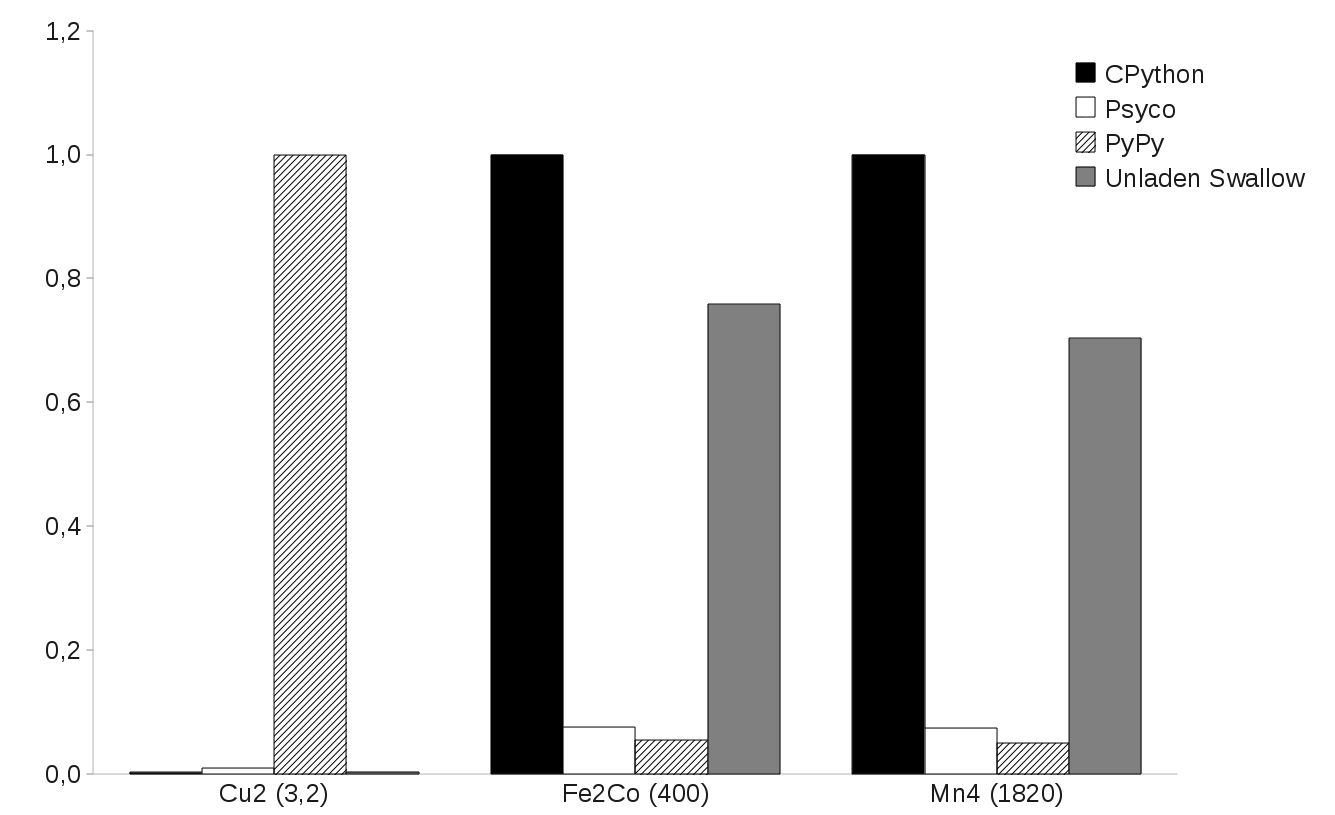
\includegraphics{03_lytvynenko_diagram1.jpg}}
\caption{Дыяграма параўнання адносных часоў выканання праграмы \progname{Mj{\"o}llnir} з рознымі JIT"=кампілятарамі (значэнні нармаваныя на час самага павольнага выканання для мадэлі (у дужках, сек)).}
\label{pic:benchmark}
\end{figure}

Такім чынам, для праграмы \progname{Mj{\"o}llnir} найбольш эфектыўным акселератарам выканання на дадзены момант з'яўляецца \progname{PyPy}, і з улікам імклівага развіцця праекта верагодным ёсць ягонае выкарыстанне ў будучыні як асноўнага (цяпер ужываецца \progname{Psyco}). \progname{Psyco} дае блізкія вынікі, \progname{Unladen Swallow} з'яўляецца неэфектыўным. Неадпаведнасць вынікаў для малой мадэлі (Cu\textsubscript{2}), верагодна, абумоўленая выдаткамі часу на JIT-кампіляцыю, якія не кампенсуюцца праз вельмі малы аб'ём разлікаў.

\begin{longtable}{|>{}c|c|c|c|}
\caption{Час выканання праграмы \progname{Mj{\"o}llnir} з рознымі JIT"=кампілятарамі, сек.}\label{tab:benchmark}\\
\hline
Мадэль&Cu\textsubscript{2}&Fe\textsubscript{2}Co&Mn\textsubscript{4}\\
\hline\endfirsthead
\hline
Мадэль&Cu\textsubscript{2}&Fe\textsubscript{2}Co&Mn\textsubscript{4}\\
\hline\endhead
Базісныя функцыі&4&432&625\\
\hline
\progname{CPython 2.6.2}&$0,0075 \pm 0,0002$&$400 \pm 7$&$1820 \pm 20$\\
\hline
\progname{Psyco 1.6}/\progname{CPython 2.6.2}&$0,0304 \pm 0,0002$&$30,5 \pm 0,3$&$134 \pm 1$\\
\hline
\progname{PyPy 1.5} &$3,2 \pm 0,1$&$21,8 \pm 0,6$&$91 \pm 2$\\
\hline
\progname{Unladen Swallow 2009Q3}&$0,010 \pm 0,005$&$303 \pm 4$&$1280 \pm 20$\\
\hline
\end{longtable}

\aknowl{Аўтар дзякуе С.\,А.~Літвіненку за каштоўныя парады пры выкананні гэтае работы.}


\newpage\begin{thebibliography}{9}

\bibitem{pDynamo} M.\,J.~Field. The pDynamo Library for Molecular Simulations using Hybrid Quantum Mechanical and Molecular Mechanical Potentials, J. Chem. Theo. Comp.,  4, 2008, 1151--1161.

\bibitem{Mjollnir} А.\,С.~Литвиненко, Е.\,А.~Михалева, С.\,В.~Колотилов, В.\,В.~Павлищук. Влияние спин"=орбитального взаимодействия на магнитную восприимчивость полиядерных комплексов 3d-металлов, содержащих ион Co\textsuperscript{2+}, Теорет. и эксперим. химия, 2010, т. 46, с. 403--409.

\bibitem{Optimize} <<Сказ о летающем змее. Агрессивная оптимизация программ на Python'e>>,  http://www.xakep.ru/magazine/xa/123/102/1.asp

\bibitem{speed} <<PyPy Speed Center: Comparison>>, http://speed.pypy.org/comparison/
\end{thebibliography}

\end{document}
